
\chapter{Introduction to the thesis}

    Bacteria and Archaea represent an abundant component of Earth's biomass, with estimates between 9.2-31.7 \num{e29} cells \cite{Kallmeyer:2012km} to 41.8-64.3 \num{e29} cells \cite{Whitman:1998tj} globally. Species diversity estimates suggest that there are close to \num{e7} different species of Bacteria and Archaea\cite{Curtis:2002dj}, although some authors suggest this number is an over-estimation \cite{Schloss:2004do}. Nevertheless, Bacteria and Archaea represent the most diverse group of organisms on Earth, and yet we have scarcely begun to characterize this diversity \cite{Wu:2009ju, Rinke:2013bt}.

    Our inability to cultivate most of the microorganisms present in the environment limits our understanding of the phylogenetic and functional diversity of microbial communities. Known as the "Great Plate-Count Anomaly" \cite{Staley:1985ww}, our current culture collections may not be representative of what can be observed in natural samples by culture-independent methods \cite{Amann:1995tw}. Most organisms are currently uncultured, due to our lack of information on their physiology and nutritional requirements \cite{Stewart:2012dd}. With new and unique cultivation methods, and information derived from genomic surveys \cite{Tyson:2005by}, we may be able to culture these organisms in the near future.
    
   Over the last decade, the development of advanced technologies and experimental methods has allowed the study of natural microbial communities via culture-independent techniques. Specifically, DNA-based methods, driven by the development of next-generation sequencing \cite{Mardis:2008fr}, have allowed the investigation of natural microbial communities without relying on cultivation. DNA-based surveys span two broad categories: marker-based analysis (such as the 16S rRNA gene) and whole genome sequencing.
    
    Marker-based analysis provides a characterization,or census, of the phylogenetic diversity present in the community, allowing for estimation of community diversity\cite{Caporaso:2011cs, Rappe:2003fc, Caporaso:2010bi} and identification of community members based on sequence similarity against a reference database  \cite{McDonald:2011hn}. This approach provides only a partial picture of the metabolic repertoire present in natural microbial communities, as it requires extrapolation of genomic data from isolated microorganisms to the entire community. Even strains with very similar 16S rRNA sequences may have different metabolic and genetic properties, which are not captured in the diversity found using a marker gene such as the 16S rRNA gene \cite{Jaspers:2004ge}.
    
    Metagenomics, also referred to as community genomics, relies on the direct sequencing of genetic material isolated from a microbial community \textit{en masse} \cite{Wooley:2010uv}, and provides the means to evaluate the phylogenetic and functional diversity of microbial populations directly from the environment. Depending on the complexity of the community under study, not all of the members of the microbial community will be observed in the sequence data, as the most abundant members will dominate the metagenomic analyses \cite{Bragg:2014kv}. Using metagenomic methods, several authors report studies of microbial communities with low to moderate species diversity  (e.g. \cite{Ugalde:2013he,Podell:2013kx,Dinsdale:2008cd,Tyson:2004bw,Brulc:2009fi}). Highly diverse communities, such as those found in soils and sediments, require high amounts of sequence information to provide a full picture of the microorganisms that are present \cite{Kakirde:2010ew}. The decrease in sequencing cost, driven by the development of novel sequencing technologies, has enhanced our ability to deeply sample complex communities using metagenomics approaches. Consequently, the challenge will be developing or acquiring the computational resources and algorithms necessary to analyze vast amounts of genetic sequence information  \cite{Pell:2012id,Kakirde:2010ew}. 
    
    Microbial communities in extreme environments, such as those associated with hypersaline habitats, represent tractable systems that can be studied using metagenomic approaches. Because of their relatively low species diversity  \cite{Andrei:2012he,Podell:2013kx,Ghai:2011hn}, it is possible to study the phylogenetic and metabolic diversity that is present in the community. In this first chapter, I provide an overview of metagenomics, with particular emphasis in assembly-based approximations, followed by an introduction into the microbiology of hypersaline environments and finally an overview of our study site, the hypersaline waters of Lake Tyrrell located in Victoria, Australia.

\section{Metagenomics}

    The study of natural microbial communities by analyzing DNA obtained directly from environmental samples was first proposed by Handelsman \textit{et al.} in 1998 \cite{Handelsman:1998tx} to access the genomic information of uncultured environmental microorganisms. The first metagenomic studies were performed by isolating DNA from environmental samples, plasmid-based cloning of this DNA and subsequence sequencing of these clones using the Sanger method \cite{Tyson:2004bw,Venter:2004hg}. Limited throughput, cloning biases, and the expesive and laborious nature of this process limited the scope of early metagenomic studies, often focused on microbial communities with low to medium species diversity \cite{Tyson:2004bw,Podell:2013kx}, or to studies aimed at describing the general functional and phylogenetic composition of a community  \cite{Venter:2004hg,Rusch:2007ez}. The development of \textit{next generation} sequencing technologies \cite{Mardis:2013gn}, removed some of these limitations, allowing for direct sequencing of DNA samples without cloning,  higher throughputs, and a lower cost per base \cite{Mardis:2013gn}. One of the remaining limitations in current technologies is the length of the sequence reads, which are not yet close to the length of reads generated by Sanger sequencing. Improvements to current methods and the development of further advanced technologies, such as single molecule sequencing \cite{Eid:2009kv} and nanopores \cite{Branton:2008fr}, holds promise to further alleviate these limitations.

Metagenomic studies are driven, in most cases, by discovery, data mining and comparative research, rather than by a specific hypothesis \cite{Wooley:2010uv}. Accordingly, both the sequence information and the contextual environmental data, or metadata, associated with a sample are of great importance, allowing for both biological and physicochemical context to be applied to the microbial community under study. These data include environmental parameters associated with a sample and procedures used to process a sample (e.g. filtration procedure, sample processing and library construction). All of these variables become highly important in the bioinformatic analysis of a sample data set\cite{Narasingarao:2012kp}.

Based on the complexity of the microbial community under study, and the choice of sampling and sequencing methods, two main approaches are used to study microbial communities using metagenomics: gene-centric and assembly-based approaches  (Figure \ref{MetagenomicComp}). 
Gene-centric studies focus on complex communities or projects with a shallow level of sequencing, where assembly of larger contiguous genome fragments from community members is not feasible given the number of reads or size of the data set obtained. . In these cases, the focus is on the phylogenetic and functional diversity as a profile of the community \cite{Ugalde:2013he,Brulc:2009fi}, and the comparison of different environments based on these profiles \cite{Dinsdale:2008cd,Willner:2009iv,Reed:2014jj}. Gene-centric studies focus on the phylogenetic and functional classification of the metagenomic reads, either by analyzing every read present in the dataset \cite{Brady:2011hi,Parks:2011bh,AmritaPati:2011ba}, or by using marker-genes as a proxy to create either taxonomic and/or functional profiles of the community \cite{Darling:2014ej,Segata:2012ba}.  One main drawbacks of this method is that community profiles are limited by the reference databases being used, which can lead to missing unique groups that are present in the microbial community under study. 

%For example, Figure \ref{CompSeqClassification} shows the results of classifying a set of metagenomic reads using two different reference databases. In this example, the query reads were obtained from a sample obtained from the hypersaline surface waters of Lake Tyrrell, sequenced on the Illumina HiSeq platform (XX reads, XX average length). Two different reference databases were used, implemented in the Phylosift \cite{Darling:2014ej} package; one where the genome of organisms know to be present in the Lake Tyrrell sample were included, and a second database where these genomes were absent. 
%\todo{Complete Phylosift results}

Assembly-based metagenomics, involves the bioinformatic assembly of the community sequence information, with the goal of recovering larger contiguous genome fragments that can improve the phylogenetic and functional classification of the organisms in the community. This approach allows the recovery of longer fragments, generate better gene models and can identify previously unknown microbial groups \cite{Narasingarao:2012kp,Podell:2013kx,Kantor:2013ir,DiRienzi:2013kx}. The information obtained from the assembled population genomes can be used to potentially guide cultivation efforts for these organisms \cite{Tyson:2005by}, in population genetic studies \cite{Simmons:2008by,Ward:2008hp,Allen:2007ju}, and provide a better picture of the interactions among the members of the microbial community \cite{Tyson:2004bw,Flowers:2013hq}. In addition, the recovery of near-complete genomes from metagenomics datasets allows for the discovery of novel functions that may be missed by viewing the unassembled sequence reads. For example, Chapter 2 of this thesis shows how the assembly of sequence reads from the Lake Tyrrell metagenome led to the discovery of a previously unknown Phylum of Archaea and to the discovery of a novel family of microbial rhodopsins, called the xenorhodopsins, and evidence that suggests its acquisition through horizontal gene transfer (Chapter 3).

Assembly-based methods are limited by the complexity of the microbial community under study, and the amount of sequencing needed to recover the genomes of the most abundant members of the community. Furthermore, some of the more rare members of the community are inaccessible by sequencing, because the most abundant organisms dominate the metagenomic dataset.  For example, estimations of the number of sequences needed to address highly diverse samples, such as from soils, show that billions of sequences are needed to be able to sample some of these most abundant organisms \cite{Howe:2014go}. Even in simpler systems, the main challenge is to classify the assembled genomic fragments into unique phylogenetic bins, each representing a different population. By combining various pieces of information, such as sample characteristics, nucleotide composition, amino acid counts, and library abundance, it is possible to classify these genomic fragments into unique populations, a process known as phylogenetic binning \cite{Podell:2013kx,Albertsen:2013gp}. Larger datasets represent a computational challenge because of the high memory requirements of short-read assembly software programs. In this case, the use of methods for digital normalization may reduce the computational problems \cite{Pell:2012id,Kakirde:2010ew}.

The work presented in this thesis describes a study of the microbial community inhabiting the hypersaline waters of Lake Tyrrell, Australia using an assembly-based approach. The combination of a relatively low-species diversity, driven by the extreme conditions found in this habitat  \cite{Andrei:2012he}, and a deep sequencing approach, allowed for the genomic reconstruction of some of the most abundant members of the community and the discovery of novel microorganisms.

%CLASSIFICATION (Using Kraken)
%This is for the datasets without the reference genomes (LT)
%17165688 sequences (1089.97 Mbp) processed in 394.493s (2610.8 Kseq/m, 165.78 Mbp/m).
%  834490 sequences classified (4.86\%)
%  16331198 sequences unclassified (95.14\%)
%  
%Minikraken
%17165688 sequences (1089.97 Mbp) processed in 57.766s (17829.5 Kseq/m, 1132.12 Mbp/m).
%  806895 sequences classified (4.70%)
%  16358793 sequences unclassified (95.30%)
%
%Classification (phylosift?)

\begin{figure}[!htbp]
	\centering
	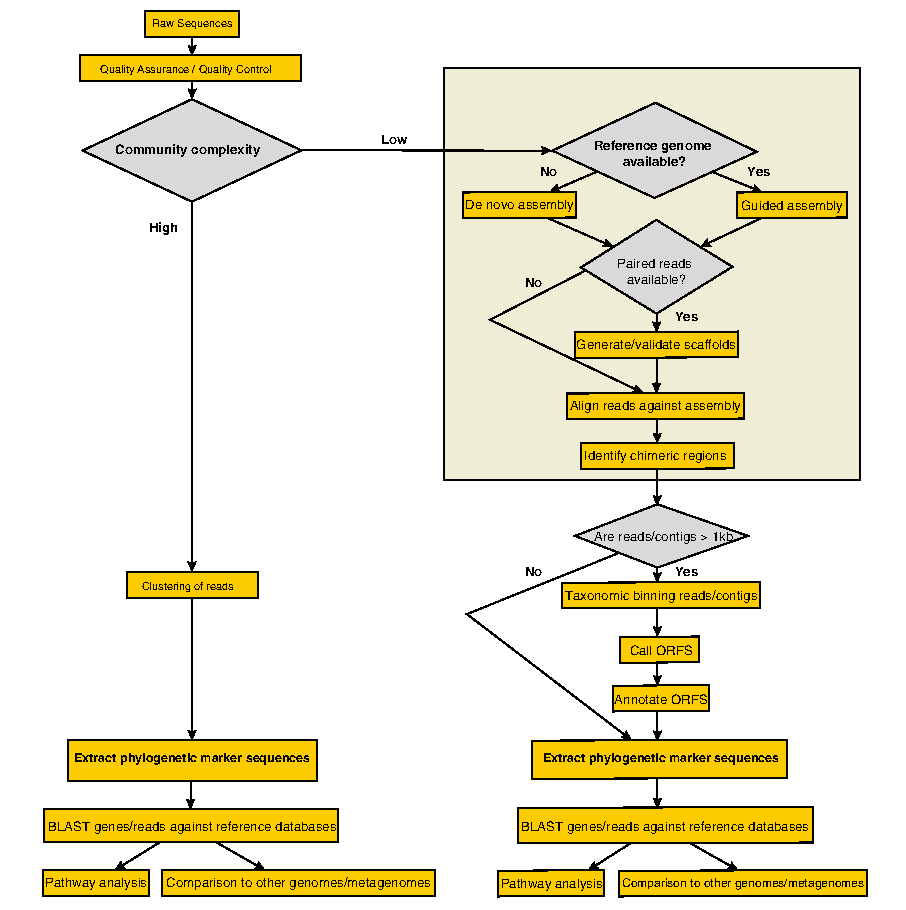
\includegraphics[width=\textwidth]{Chapter1/Figures/Metagenomics_GeneCentric_vs_Assembly.pdf}
	\caption{Diagram comparing two possible approaches for the analysis of metagenomic data from natural microbial communities. Figure from Bragg and Tyson, 2014 \cite{Bragg:2014kv}.}
	\label{MetagenomicComp}
\end{figure}

%\begin{figure}[!htbp]
%	\centering
%	*
%	\caption{Comparison of a set of reads (Illumin XXbp, total of XX reads) classified using Phylosift? with two different reference databases. The first case shows the reads classified in abscence of any reference genomes, the second one where reference genomes obtained through metagenomics \cite{Narasingarao:2012kp,Podell:2013kx} are included in the database}
%	\label{CompSeqClassification}
%\end{figure}

\section{Microbial communities in hypersaline environments}

Hypersaline habitats are found worldwide, in a variety of natural and man-made environments. Examples include salt lakes, saline soils, salt flats, solar salterns, brine pools, salted foods, and fermented foods \cite{Oren:2002vw}. Aquatic hypersaline systems are the most studied, and are either of marine origin (thalassohaline), or formed by the dissolution of mineral salt deposits (athalassohaline). 

Within these saline systems, a variety of microbial species are adapted to these environments. Moderate halophiles can beare found between 30-150 g/L NaCl, while extreme halophiles exist in the range of 150-300 g/L NaCl  \cite{Andrei:2012he}. In addition to the high NaCl concentrations, other salts are also important to consider when measuring the ionic composition of these systems, including Mg\textsuperscript{2+} and Ca\textsuperscript{2+}, which can inßuence the microbial community in these habitats  \cite{McGenity:2000ts,Podell:2013fp} (Figure \ref{IonicComposition}).

Genera from both the Bacteria and the Archaea exist in moderate and extreme saline systems. Within the Archaea, the phylogenetic diversity appears to be limited to the \textit{Euryarchaeota}, specifically in the classes \textit{Halobacteria} and \textit{Methanomicrobia} (Table \ref{TableArchaea}) \cite{Ventosa:2012wo}. The discovery of the \textit{Nanohaloarchaea} (described in Chapter 2, and \cite{Narasingarao:2012kp}), a novel Class, within the Euryarchaeota,, in globally dispersed hypersaline systems expanded our understanding of the phylogenetic diversity of halophilic Archaea \cite{Narasingarao:2012kp}. Recently, a phylogenomic analysis of novel archaeal groups, isolated via single-cell genomics, suggested that the \textit{Nanohaloarchaea} are a new phylum, sister to the \textit{Euryarchaeota} \cite{Rinke:2013bt}, although more work (and more genomes and isolates) is needed to fully resolve the phylogenetic relationships between these groups \cite{Williams:um}.

Even within the \textit{Halobacteria}, novel taxonomic groups remain unidentified. Our group recently described the genome of a newly isolated halophilic Archaea,  \textit{Candidatus} Halobonum tyrrellensis strain G22 \cite{Ugalde:2013hb}, which phylogenetic analysis suggests is a new genus within the \textit{Halobacteria} (Appendix \ref{G22Genome}). Analysis of the 16S rRNA gene, and a phylogenomic approach using the markers genes implemented in the software, PhyloPhlan, has further supported this phylogenetic placement (Figures \ref{G22_16Stree} \& \ref{G22_PhyloPhlanTree}).

The phylogenetic breadth of bacterial species found in saline systems is wider than that of Archaea (Table \ref{TableBacteria}). In moderate saline environments, Bacteria are more abundant than Archaea \cite{Oren:2008ej,Ghai:2011hn,Ghai:2012fb,Casamayor:2002tf}, but as salinity increases, Archaeal groups become more abundant \cite{Ghai:2011hn,Casamayor:2002tf,Mutlu:2008dk}. One of the most abundant bacterial species found in extreme hypersaline systems is \textit{Salinibacter ruber} \cite{Anton:2008eb}. This bacterium shares many phenotypic characteristics with halophilic Archaea \cite{Oren:2013gy}, and multiple gene clusters appear to have been acquired via horizontal gene transfer from the Archaea \cite{Mongodin:2005ie}.

Viruses are also very abundant in hypersaline systems, with reports of counts of at least \num{e7} viral-like particles per mL \cite{DyallSmith:2003eu}. Viruses could be playing a dual role in these systems; as predators, contributing to the cycling of nutrients through cell lysis; and as a form of information storage, by providing access to an auxiliary gene pool that can be utilized by other microorganisms \cite{Lindell:2005gz,Williamson:2008vs,Hurwitz:2013gl}.  Studies of viral dynamics in hypersaline systems have showed that they play a fundamental role in shaping the population structure of microbial communities \cite{RodriguezBrito:2010in,RodriguezValera:2009cr}.

Microorganisms that live in hypersaline systems require particular physiological strategies to deal with the high salt concentrations and the potential osmotic pressure gradient that can generate across the cell membrane. Two different osmotic adaptation strategies can be found in halophiles: a salt-in strategy, which involves the accumulation of inorganic ions in the cytoplasm; and a salt-out strategy, that involves pumping ions out the cell and the accumulation of compatible solutes in the cytoplasm \cite{Oren:2013bc}. The salt-in strategy is found in the archaeal populations, specifically within the Order \textit{Halobacteriales}, in Bacteria of the Order \textit{Halanerobiales} and in \textit{S. ruber} \cite{Oren:2013bc}. These organisms accumulate inorganic ions, such as K\textsuperscript{+} and Cl\textsuperscript{-}, which requires special enzymatic adaptations reflected through protein amino acid compositional changes that favor acidic amino acids, such as glutamate and aspartate. Based on their amino acid composition profiles, it has been suggested that the uncultured members of the Class \textit{Nanohaloarchaea} also utilize this strategy. The salt-out strategy is found in most of the halophilic Bacteria and halophilic methanogenic Archaea  \cite{Oren:2013bc}. These organisms have outward-directed sodium transporters that pump the Na\textsuperscript{+} ions out of the cytoplasm, but more importantly, they accumulate a large number of organic solutes to mantain the osmotic potential in the cytoplasm \cite{Oren:2013bc}.

Halophilic microorganisms show a diverse suite of metabolic capabilities. Several dissimilatory metabolic pathways have been described in halophiles (Figure \ref{HaloMetabolis}) across a wide range of salinity concentrations. The majority of bacterial and archaeal groups isolated from hypersaline sites are aerobic chemoorganotrophs. In addition, as oxygen has a low solubility in salt saturated brines \cite{Sherwood:1991tg}, several anaerobic energy pathways are available, including electron acceptor substrates such as nitrate, fumarate, and dimethyl sulfoxide \cite{Oren:2008ej,Oren:2013bc}. Primary productivity in saline systems varies according to the salinity. In moderate saline environments (between 100 to 250 g/L), primary productivity occurs in microbial mats dominated by members of the \textit{Cyanobacteria};  in high salt environments, the primary producers are planktonic algae of the genus \textit{Dunaliella} \cite{Oren:2009el}.

Another important characteristic of halophilic organisms, particularly among the halophilic Archaea, is the presence of microbial rhodopsins, photoactive proteins found in all three domains of life. Rhodopsins serve as light-driven proton pumps (bacteriorhodopsin), chloride pumps (halorhodopsin), or phototactic and photophobic receptors (sensory rhodopsins) \cite{Brown:2013ic}. Halorhodopsins and sensory rhodopsins appear to be limited in their distribution to the \textit{Halobacteria}, with just a few examples found in other organisms \cite{Sharma:2006kn}. Chapter 3 describes the discovery a novel type of microbial rhodopsin, called the xenorhodopsin, which was found in the genome of the \textit{Nanohaloarchaea}, and that appear to broadly dispered via horizontal gene transfer between Archaea and Bacteria (although it is not possible yet to establish the directionality of acquisition).Indeed, the closest homolog to the Nanohaloarchaea xenorhodopsin is a putative sensory rhodopsin found in the cyanobacterium \textit{Anabaena} sp. PCC 712 \cite{Vogeley:2004vh,Ugalde:2011fw}.

Even in highly characterized microbial communities  \cite{Oren:2008ej,Oren:2012bg}], recent studies using culture independent techniques, such as metagenomics and single-cell genomics, recovered novel microbial groups \cite{Narasingarao:2012kp,Ghai:2011hn,LopezPerez:2013db}. The limited microbial diversity, driven by extreme salinity systems, makes them ideal model systems to study microbial diversity using metagenomic methods. We can fully characterize a microbial community using deep-sequencing approaches, with the goal to reconstruct the genomes of each member of the community. Through this approach, we identify not only the functional and phylogenetic diversity of the community, but also the association of such functions to members of the community. Lastly, it allows for the study of population genetics within the community, with the goal of understanding how these organisms adapt and respond to variations in the environment.

It is important to highlight that other saline ecosystems have been studied using metagenomic approaches. Prior hypersaline metagenomic studies have focused on the population genomics of single species, such as \textit{Haloquadratum walsbyi} \cite{Legault:2006kh} and \textit{Salinibacter ruber} \cite{Pasic:2009bo}, or on the dynamic changes of the microbial and viral diversity over salinity gradientes and over time \cite{Willner:2009iv,RodriguezBrito:2010in}. Only recent studies have explored the microbial and viral diversity of these systems by using assembly-based metagenomics and single-cell genomics approaches \cite{Narasingarao:2012kp,Podell:2013kx,Ghai:2011hn,Ghai:2012fb,Emerson:2012gh,Emerson:tk}.

%FIGURE, G22 16S TREE
\begin{figure}[!htbp]
	\centering
	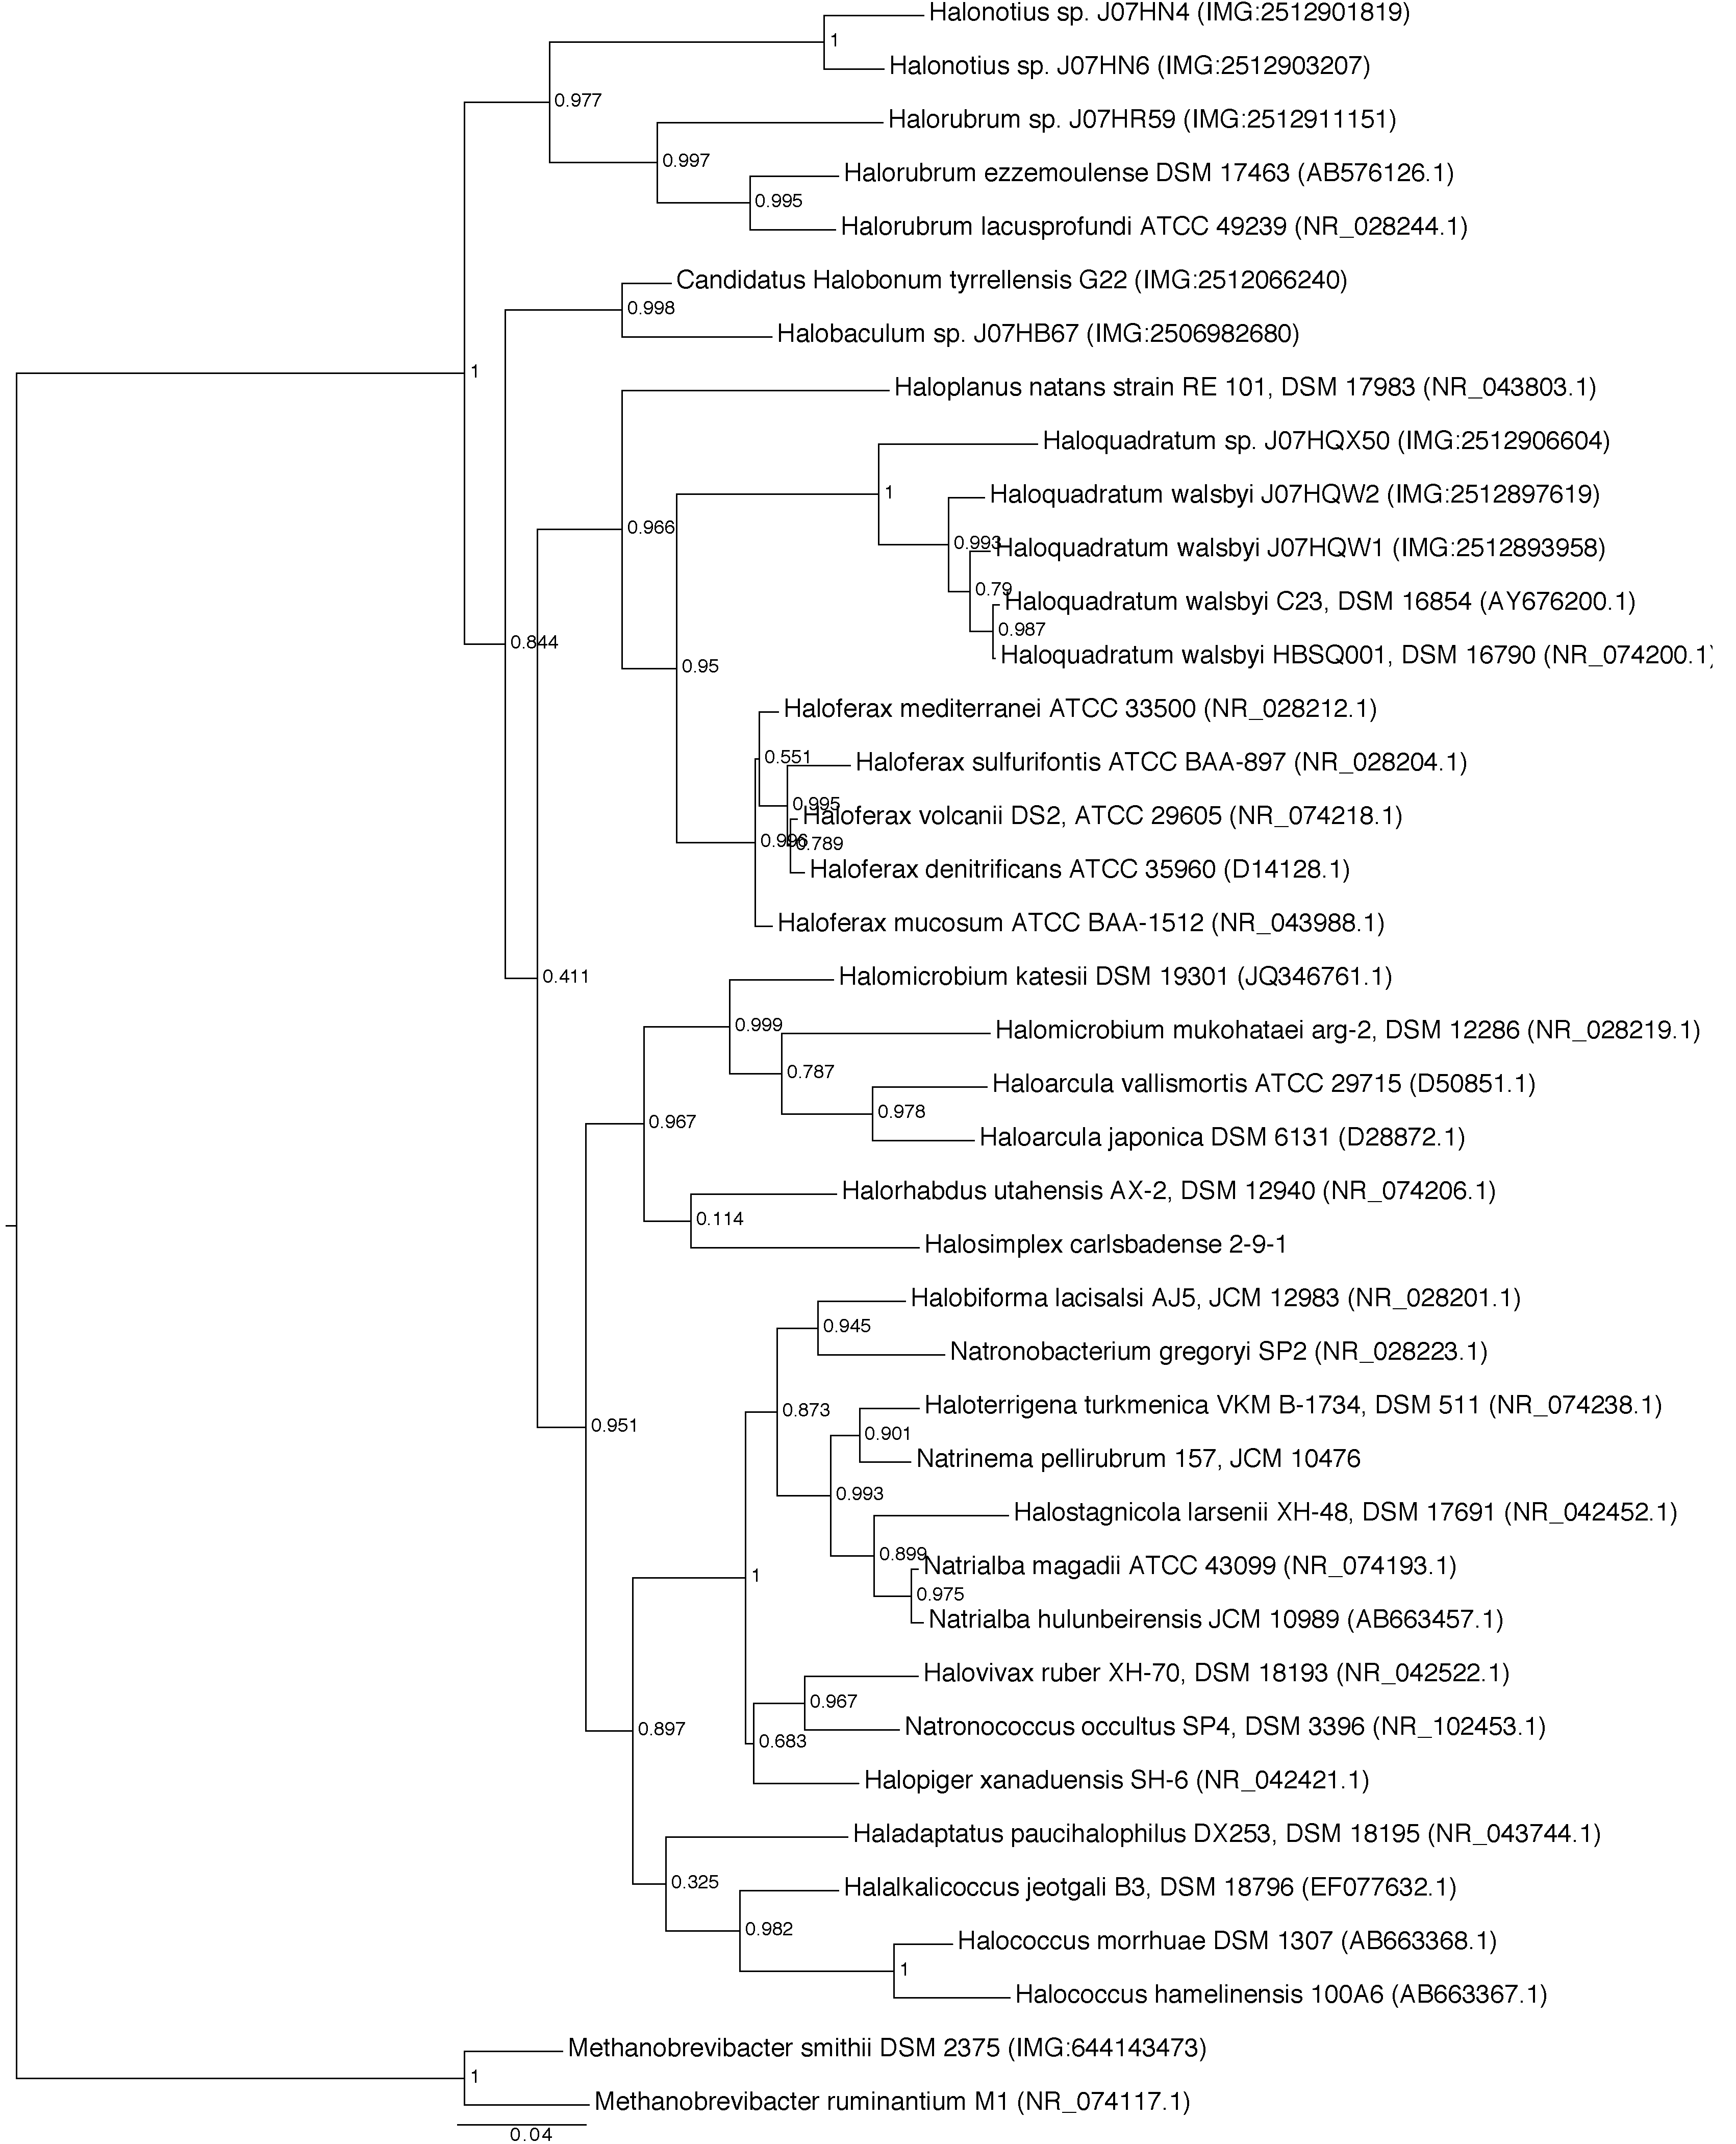
\includegraphics[width=\textwidth]{Chapter1/Figures/HaloG22_16S_v2-2.pdf}
	\caption{Phylogenetic tree of \textit{Candidatus} Halobonum tyrrellensis G22 and related microorganisms, based on 16S rRNA sequences.}
	\label{G22_16Stree}
\end{figure}

%FIGURE, G22, PHYLOPHLA TREE
\begin{figure}[!htbp]
	\centering
	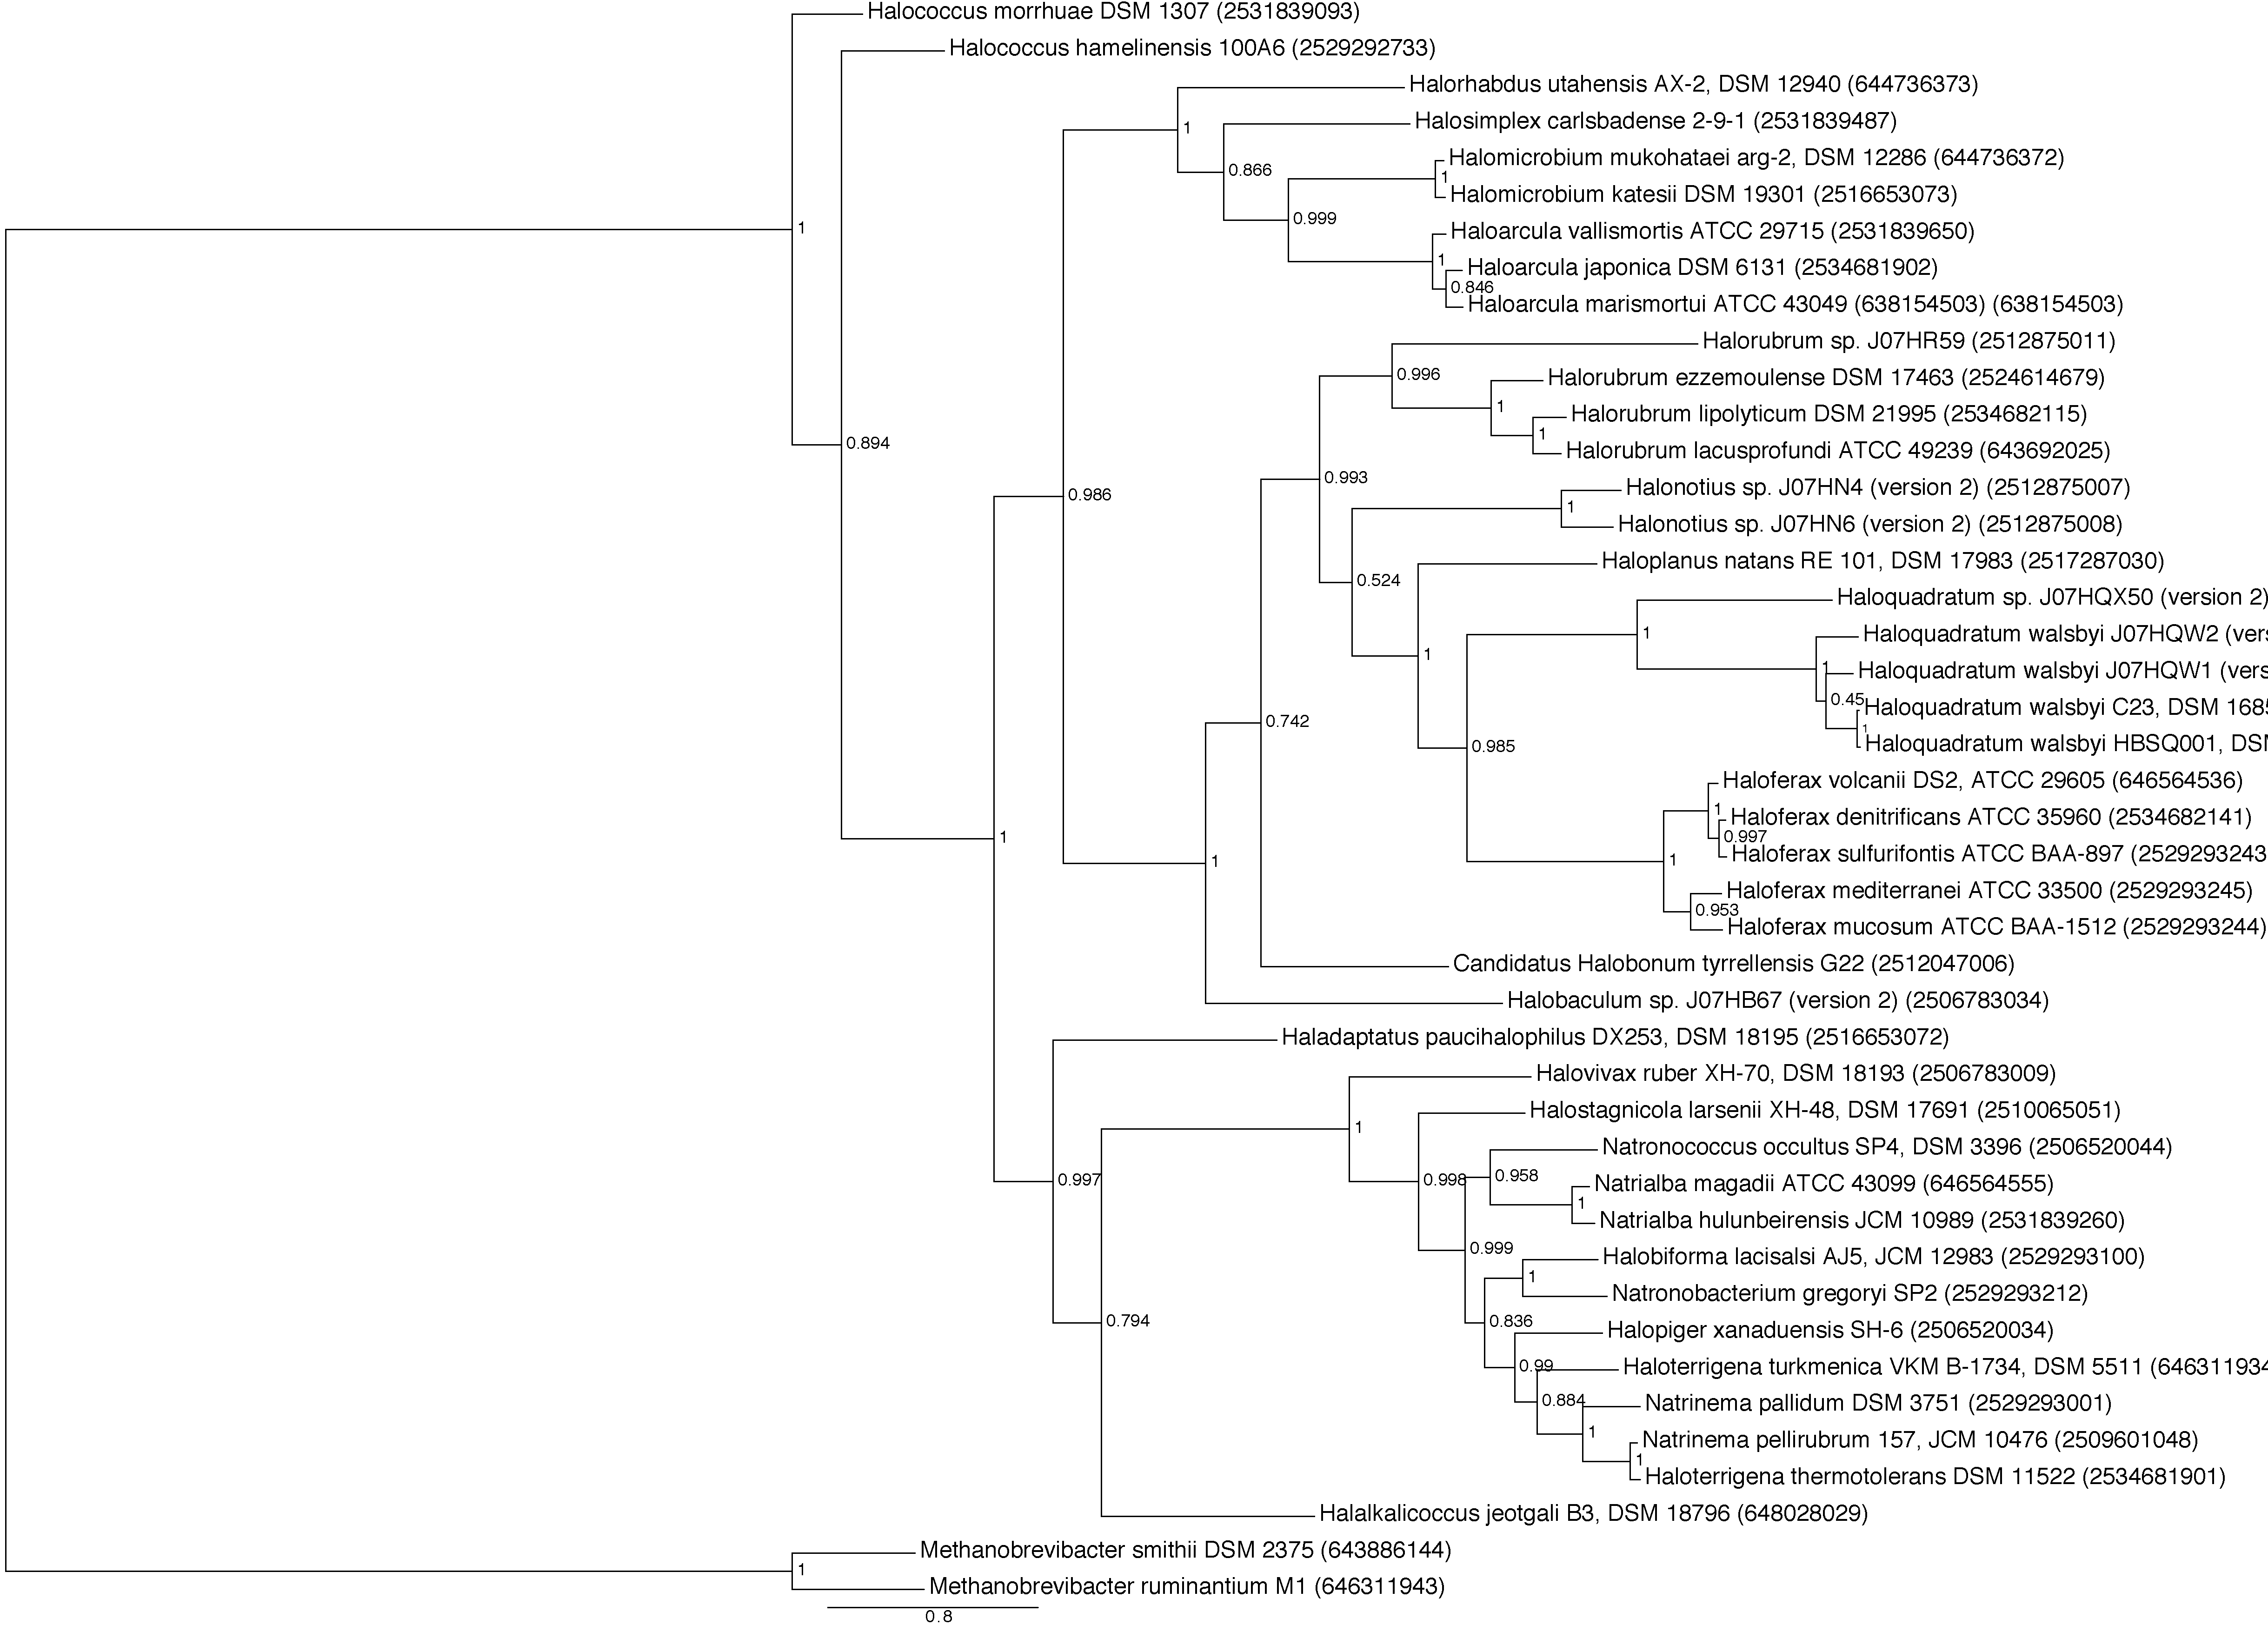
\includegraphics[width=\textwidth]{Chapter1/Figures/HaloG22_v6.pdf}
	\caption{Phylogenetic tree of \textit{Candidatus} Halobonum tyrrellensis G22 and related microorganisms, based on phylogenetic marker sequences implemented in the Phylophlan software \cite{Segata:2013hb}}
	\label{G22_PhyloPhlanTree}
\end{figure}

%FIGURE IONIC COMPOSITION
\begin{figure}[!htbp]
	\centering
	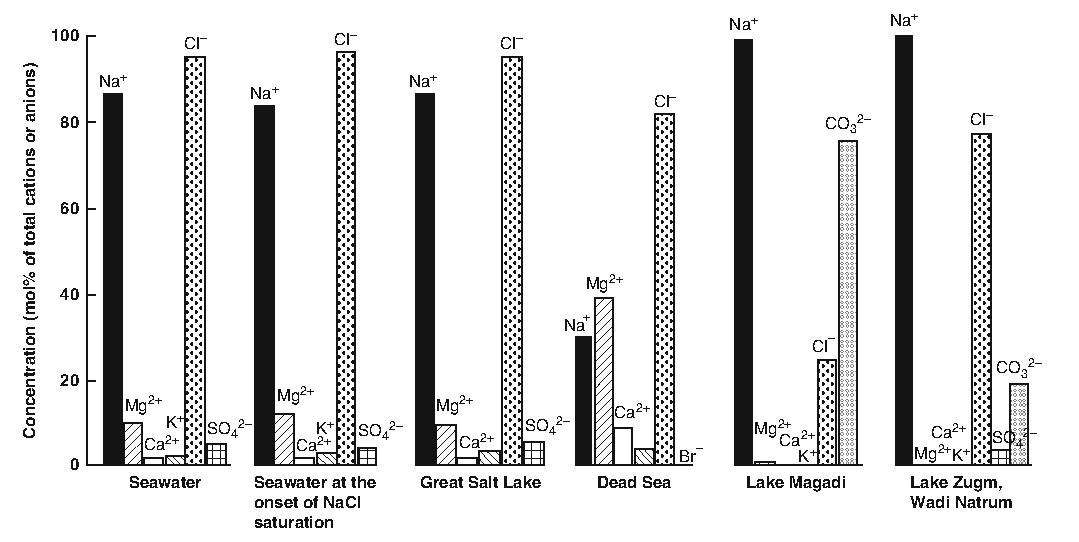
\includegraphics[width=\textwidth]{Chapter1/Figures/IonicComposition.pdf}
	\caption{Ionic composition of several aquatic systems. Figure from Oren, 2013. \cite{Oren:2013bc}}
	\label{IonicComposition}
\end{figure}

%FIGURE IONIC COMPOSITION
\begin{figure}[!htbp]
	\centering
	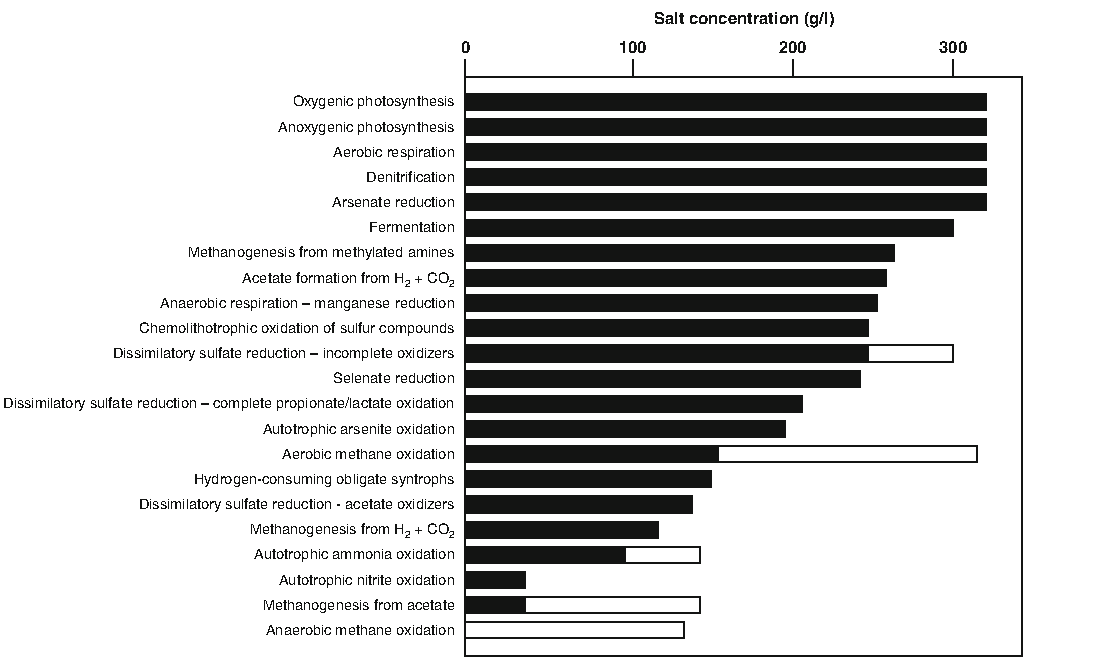
\includegraphics[width=\textwidth]{Chapter1/Figures/HaloMetabolism.pdf}
	\caption{Salt concentration limits for some microbial metabolic processes. Black bars indicate information based on laboratory studies, while white bars indicate activities measured in natural microbial communities. Figure from Oren, 2013 \cite{Oren:2013bc}.}
	\label{HaloMetabolis}
\end{figure}


%TABLE, ARCHAEA DIVERSITY
\begin{table}[!htdp]
\caption{Halophilic Archaea, modified from \cite{Ventosa:2012wo} to include the recently discovered \textit{Nanohaloarchaea} \cite{Narasingarao:2012kp}.}
\begin{center}

\resizebox{\textwidth}{!}{%
\begin{tabularx}{\textwidth}{p{3cm} p{3cm} X}
\hline
\textbf{Phylum} & \textbf{Class} & \textbf{Genera} \\
\hline
\textit{Euryarchaeota} & \textit{Halobacteria} & \textit{Halobacteria, Haladaptatus, Halalkalicoccus, Halarchaeum, Haloarcula, Halobaculum, Halobiforma, Halococcus, Haloferax, Halogeometricum, Halogranum, Halomicrobium, Halonotius, Halopelagius, Halopiger, Haloplanus, Haloquadratum, Halorhabdus, Halorubrum, Halorussus, Halosarcina, Halosimplex, Halostagnicola, Haloterrigena, Halovivax, Natrialba, Natrinema, Natronoarchaeum, Natronobacterium, Natronococcus, Natronolimnobius, Natronomonas, Natronorubrum, Salarchaeum} \\
\cline{2-3} 
& \textit{Methanomicrobia} & \textit{Methanohalobium, Methanocalculus, Methanohalohilus, Methanosalsum} \\
\hline
\textit{Nanohaloarchaea} &  & \textit{Nanosalina, Nanosalinarum} \\
\end{tabularx}
}

\end{center}
\label{TableArchaea}
\end{table}




%TABLE BACTERIA DIVERSITY
\begin{center}

\begin{longtable}{p{3cm} p{4.5cm} p{5.5cm}}
\label{TableBacteria}\\
\caption{Halophilic Bacteria, modified from \cite{Ventosa:2012wo}.}\\

\hline
\textbf{Phylum} & \textbf{Class} & \textbf{Genera} \\
\hline
\endfirsthead

\multicolumn{3}{c}%
{\tablename\ \thetable\ -- \textit{Continued from previous page}} \\
\hline
\textbf{Phylum} & \textbf{Class} & \textbf{Genera} \\
\hline
\endhead

\hline \multicolumn{3}{r}{\textit{Continued on next page}} \\
\endfoot
\hline
\endlastfoot


\textit{Actinobacteria} & \textit{Actinobacteria} & \textit{Actinopolyspora, Amycolatopsis, Georgenia, Corynebacterium, Haloactinobacterium, Haloactinopolyspora, Haloechinothrix, Haloglycomyces, Nesterenjonia, Nocardiopsis, Haloactinospora, Streptomonospora, Isoptericola, Prauserella, Saccharomonospora, Saccharopolyspora} \\
\hline

\textit{Bacteroidetes} & \textit{Bacteroidia} & \textit{Anaerophaga} \\
\cline{2-3}

& \textit{Flavobacteria} & \textit{Gramella, Psychroflexus} \\
\cline{2-3}
& \textit{Sphingobacteria} & \textit{Salinibacter, Salisaeta} \\
\hline

\textit{Cyanobacteria} & & \textit{Rubidibacter, Prochlorococcus, Halospirulina} \\
\hline

\textit{Firmicutes} & \textit{Bacilli} & \textit{Alkalibacillus, Aquisalibacillus, Bacillus, Filobacillus, Gracilibacillus, Halalkalibacillus, Halolactibacillus, Halobacillus, Jeotgalibacillus, Lentibacillus, Oceanobacillus,Ornithinibacillus, Paraliobacillus, Piscibacillus, Pontibacillus, Salimicrobium, Salinibacillus, Salirhabdus, Salsuginibacillus, Sediminibacillus, Salinicoccus, Tenuibacillus, Thalassobacillus, Virgibacillus} \\
\cline{2-3}
& \textit{Clostridia} & \textit{Acetohalobium, Halanaerobacter, Halanaerobium, Halobacteroides, Halocella, Halonatronum, Halothermothrix, Natranaerobius, Natrionella, Natronovirga, Orenia, Selenihalanaerobacter, Sporohalobacter} \\
\hline

\textit{Proteobacteria} & \textit{Alphaproteobacteria} & \textit{Antarctobacter, Citreimonas, Dichotomicrobium, Fodinicurvata, Hwanghaeicola, Hyphomonas, Jannaschia, Maribaculum, Maribius, Marispirillum, Methylarcula, Oceanibulbus, Oceanicola, Palleronia, Paracoccus, Ponticoccus, Rhodobium, Rhodotalassium, Rhodovibrio, Rhodovulum, Roseicitreum, Roseinatronobacter, Roseisalinus, Roseospira, Roseovarius, Salinihabitans, Salipiger, Sediminimonas, Shimia, Sulfitobacter, Tropicibacter, Woodsholea, Yangia} \\
\cline{2-3}
& \textit{Gammaproteobacteria} & \textit{Aidingimonas, Alcanivorax, Alkalilmnicola, Alteromonas, Aestuariibacter, Aquisalimonas, Arhodomonas, Carnimonas, Chromohalobacter, Cobetia, Ectothiorhodspira, Ectothiorhodosinus, Glaciecola, Gilvimarinus, Haliea, Halochromatium, Halomonas, Halorhodospira, Halospina, Halothiobacillus, Idiomarina, Kushneria, Marichromatium, Marinobacter, Marinobacterium, Melitea, Methylohalomonas, Microbulbifer, Modicisalibacter, Nitrincola, Oleispira, Pseudidiomarina, Pseudoaltermonas, Psychromonas, Pseudomonas, Saccarospirillum, Salicola, Salinicola, Salinisphaera, Salinivibrio, Thioalkalibacter, Thioalkalivibrio, Thiohalobacter, Thiohalorhabdus, Thiohalocapsa, Thiohalomonas, Thiohalophilus, Thiohalospira, Thiomicrospira} \\
\cline{2-3}
& \textit{Deltaproteobacteria} & \textit{Desulfocella, Desulfohalobium, Desulfonatronospira, Desulfosalsimonas, Desulfovermiculus, Desulfovibrio, Desulfurivibrio} \\
\cline{2-3}
& \textit{Epsilonproteobacteria} & \textit{Arcobacter, Sulfurimonas, Sulfurovum} \\
\hline

\textit{Spirochaetes} & \textit{Spirochaetes} & \textit{Spirochaeta} \\
\hline

\textit{Tenericutes} & \textit{Mollicutes} & \textit{Haloplasma} \\
\hline

\textit{Thermotogae} & \textit{Thermotogae} & \textit{Petrotoga} \\

\end{longtable}

\end{center}





\section{Lake Tyrrell, Australia, as a model ecosystem}

Lake Tyrrell, Victoria, Australia, is located in the center of the Murray Basin Plains (Figure \ref{LT_map}), in a region with a semi-arid climate, average rainfall of 300 mm/year, and an evaporation rate of ~2000 mm/year  \cite{Macumber:1992ty}. The lake is considered an acid-hypersaline system, where low-pH, oxygenated, saline, metal-rich groundwater from springs is evapo-concentrated and mixed with near-neutral pH waters, rich in sulfides \cite{Long:1992ie}. The lake shows seasonal salinity variations. During winter, the salt content is approximately  \textgreater 250 g/L; in summer, due to water evaporation, the residual brines reach concentrations \textgreater 330 g/L \cite{Macumber:1992ty}.

Lake Tyrrell has been described and studied in detail in terms of its hydrological and geochemical features  \cite{Long:1992ie,Macumber:1992ty,Jones:2006jn}], making it a great candidate for microbiological characterization. Recent projects have used a diverse array of microbiological techniques to study the microbial diversity of Lake Tyrrell, including Eukaryotes \cite{KarlaBHeidelberg:2013jc}, Archaea and Bacteria \cite{Podell:2013kx,Narasingarao:2012kp,Ugalde:2013hb}, and Viruses \cite{Emerson:2012gh,Emerson:tk}. Future work will combine the metagenomic, proteomic, and available geochemical information to provide a more integrative description of the interactions between microbes, viruses, and the environment. 

In this thesis, we explore the microbial diversity of the Lake Tyrrell ecosystem, based on the data generated through a metagenomic study. In particular, our study highlights how, by assembling metagenomic data, we obtain a more complete picture of the microbial diversity present in the community, and also how we can exploit this information to obtain a broad picture of the phylogenetic and functional diversity, and to explore in detail the genetic diversity of the members of the microbial community.

\textbf{Chapter 2} describes how the assembly of metagenomic datasets allowed the recovery and identification of novel microbial groups that are abundant in the hypersaline waters of Lake Tyrrell, and other hypersaline ecosystems. Using additional metadata, such as size fractionation, sequence nucleotide composition, and phylogenetic binning, two near-complete genomes from a novel Class of Archaea, the \textit{Nanohaloarchaea}, were recovered from the metagenomic samples. . This chapter represents work that has already been published  \cite{Narasingarao:2012kp}. My role, in this study was in the classification of sequences into phylogenetic groups using statistical approaches, such as non-metric multidimensional scaling, and exploring the functional diversity of the two novel genomes.

\textbf{Chapter 3} corresponds to the bioinformatic analysis and description of a novel type of microbial rhodopsin, xenorhodopsin, identified from the genomes of the Nanohaloarchaea.The results convey how this rhodopsin appears to be a new class of microbial rhodopsin based on phylogenetic analysis and on the presence of unique amino acid signatures. This work has already been published \cite{Ugalde:2011fw}, where I was the lead author of the study. 

\textbf{Chapter 4} describes the assembly of several genomes from the Lake Tyrrell metagenome, based on the combination of assembly-based approaches and metadata. These results provide a framework for future analyses of this ecosystem, providing a set of habitat-specific genomes, including phylogenetic, functional, and genetic diversity. This work is already published \cite{Podell:2013kx}. My role in this study was developing the methods for classification of the assembled scaffolds into different phylogenetic groups and developing novel visualization and analysis approaches to compare the functional repertoire of community members.

\textbf{Chapter 5}, leverages the assembled habitat-specific genomes, and describes a bioinformatic approach for the analysis of genetic diversity using metagenomic approaches. Using this framework, a deep-sequencing approach was used to characterize the population composition and genetic heterogeneity of two different temporal samples (Summer and Winter) from the microbial members of the Lake Tyrrell community.

%FIGURE LT MAP
\begin{figure}[!htbp]
	\centering
	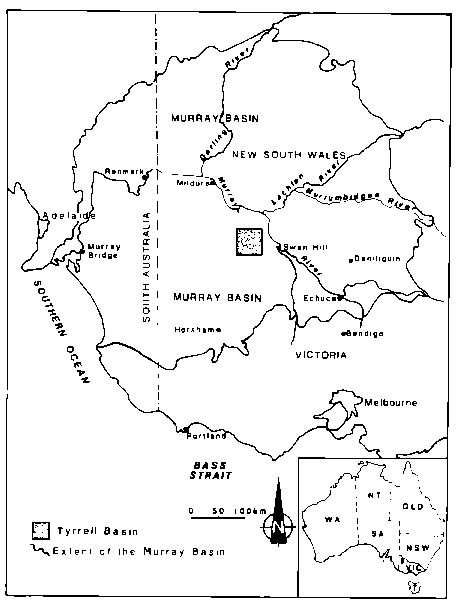
\includegraphics[width=\textwidth]{Chapter1/Figures/LT_Map.pdf}
	\caption{Location of Lake Tyrrell in the southeastern region of Australia. Figure from Macumber, 1992. \cite{Macumber:1992ty}.}
	\label{LT_map}
\end{figure}

